\DailyTitle{6411 Log (November 29, 2010)}

\DailySection{Hcal toy studies during the past few days}

What was done:

\begin{enumerate}
\item Generate single-pulse toy samples with different timing spread and pedestal fluctuation
\item Generate dual-pules toy samples with different time distance and relative size
\item Mixed data with data with different time distance.  Done: Jet+MB, Jet+Jet, Jet+MultiJet, Noise+MB, Noise+Jet, Noise+MultiJet.  Time difference: -100ns, -75ns, -50ns, 50ns, 75ns, 100ns
\end{enumerate}


Short summary on what is observed:

\begin{enumerate}
\item Single Pulse Toy: Pedestal level in slopes affects low-energy pulse but not the higher energy ones.  Figure \ref{Figure_6411_TimeAndPedestalScanLeftSlope}.
\item Single Pulse Toy: Timing spreads out slope distributions.  Figure \ref{Figure_6411_TimeAndPedestalScanLeftSlope}.
\item Dual Pulse Toy: Edge in linear and spike discriminator moves.  Figures \ref{Figure_6411_ToysAllChargeLambdaLinear} and \ref{Figure_6411_ToysAllChargeLambdaRMS8Max}.
\item Dual Pulse Toy: Slow-dropping and slow-rising slopes not usable.  Fast dropping one is useful however.  The edge seems to be independent to out-of-time pileup.
Figures \ref{Figure_6411_ToysAllChargeLeftSlope}, \ref{Figure_6411_ToysAllChargeRightSlope} and \ref{Figure_6411_ToysAllChargeRightSlopeZoomIn}.
\item Dual Pulse Toy: Structure in the slopes.  Upper-right direction: out-of-time pulse height.  Upper-left: in-time pulse height.  Is it okay to throw away hits with huge out-of-time pileup?  It will be random and it will be extremely rare.
Figure \ref{Figure_6411_Toys75LateScanRightSlope}.
\item Dual Pulse Toy: Updated signal hypothesis.  Improves things.  Figures \ref{Figure_6411_ToysAllChargeLambdaDLinear} and \ref{Figure_6411_ToysAllChargeLambdaDRMS8Max}
\item Jet+Jet: Things look better with the updated signal hypothesis.
Figures \ref{Figure_6411_MixJetOnJetLambdaLinear}, \ref{Figure_6411_MixJetOnJetLambdaDLinear}, \ref{Figure_6411_MixJetOnJetLambdaRMS8Max} and \ref{Figure_6411_MixJetOnJetLambdaDRMS8Max}
\item Jet+Jet: Lower edge of right slope is indeed invariant.  Figure \ref{Figure_6411_MixJetOnJetRightSlopeZoomIn}.
\item Noise+Jet: The fast-dropping population is still there.  Good.  Figure \ref{Figure_6411_MixNoiseOnJetRightSlopeZoomIn}.
\item X+MB: Minimum bias events are boring.  It's too soft so we won't see much.  Figure \ref{Figure_6411_MixJetOnMBRightSlope}.
\item X+MultiJet: The hardness of rechits in jet dataset and multijet dataset is roughly the same.  The multijet dataset has more rechits per event on average though.
But since only pulse-by-pulse mixing is considered here, the distributions are exactly the same as the X+Jet distributions.  Figure \ref{Figure_6411_MixJetOnJetLeftSlope} and \ref{Figure_6411_MixJetOnMultiJetLeftSlope}.
\end{enumerate}

\begin{figure}
   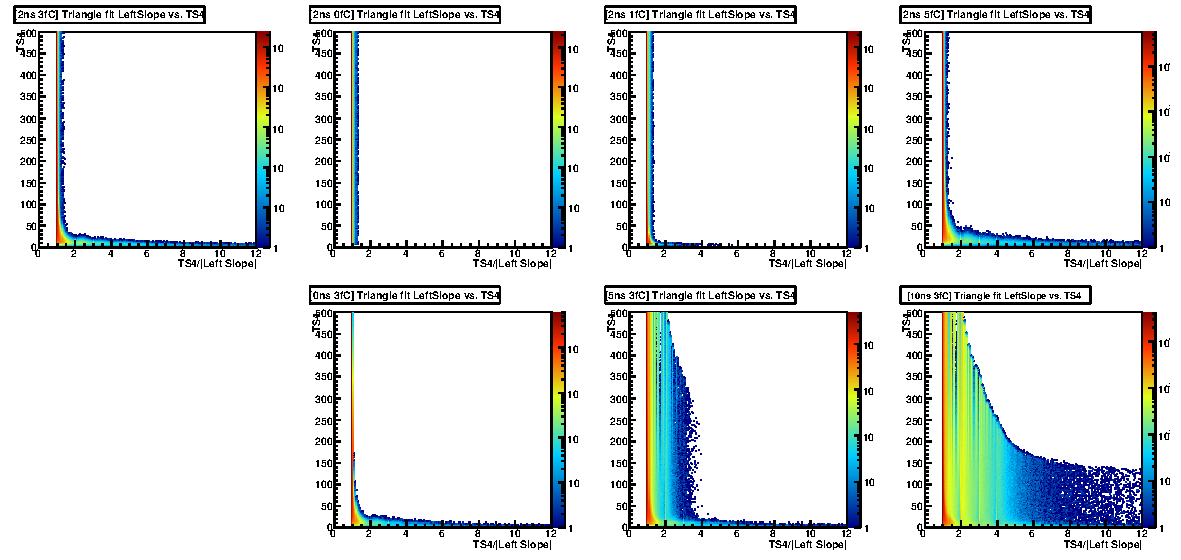
\includegraphics[width=120mm]{DailyLog/6411/6411_TimeAndPedestalScanLeftSlope.pdf}
   \caption{Time and pedestal scan for single-pulse toys}
   \label{Figure_6411_TimeAndPedestalScanLeftSlope}
\end{figure}

\begin{figure}
   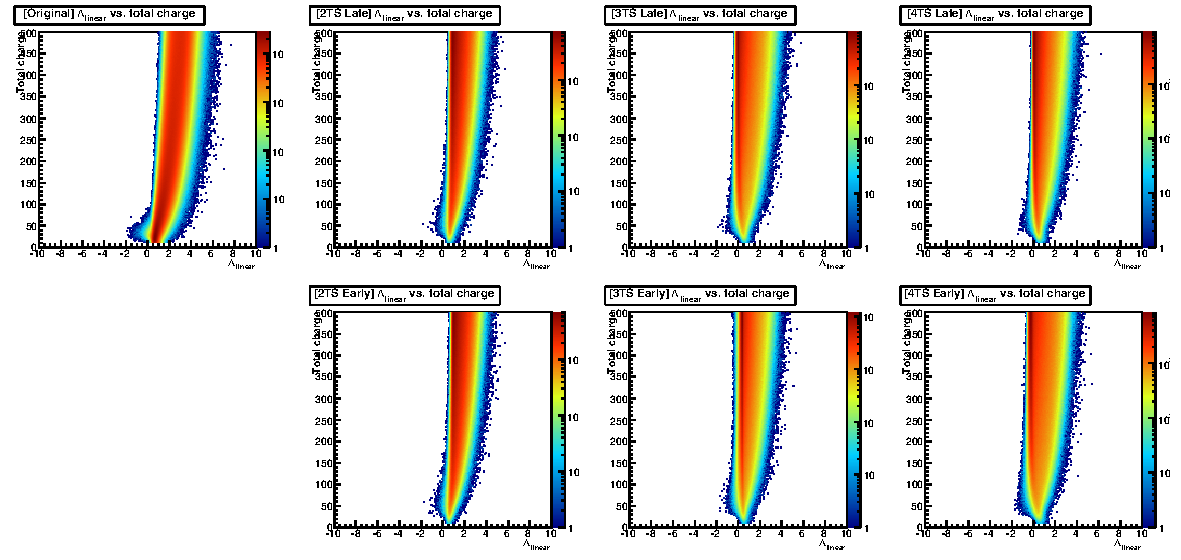
\includegraphics[width=120mm]{DailyLog/6411/6411_ToysAllChargeLambdaLinear.pdf}
   \caption{With mixing, edge in $\Lambda_{linear}$ moves (Toy)}
   \label{Figure_6411_ToysAllChargeLambdaLinear}
\end{figure}

\begin{figure}
   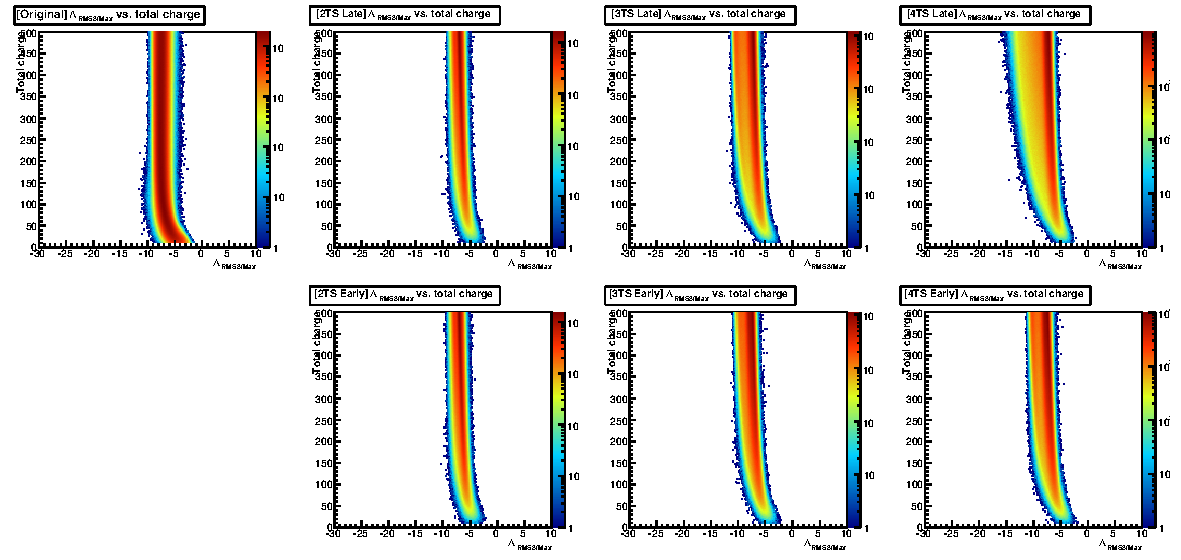
\includegraphics[width=120mm]{DailyLog/6411/6411_ToysAllChargeLambdaRMS8Max.pdf}
   \caption{With mixing, edge in $\Lambda_{RMS8/Max}$ moves (Toy)}
   \label{Figure_6411_ToysAllChargeLambdaRMS8Max}
\end{figure}

\begin{figure}
   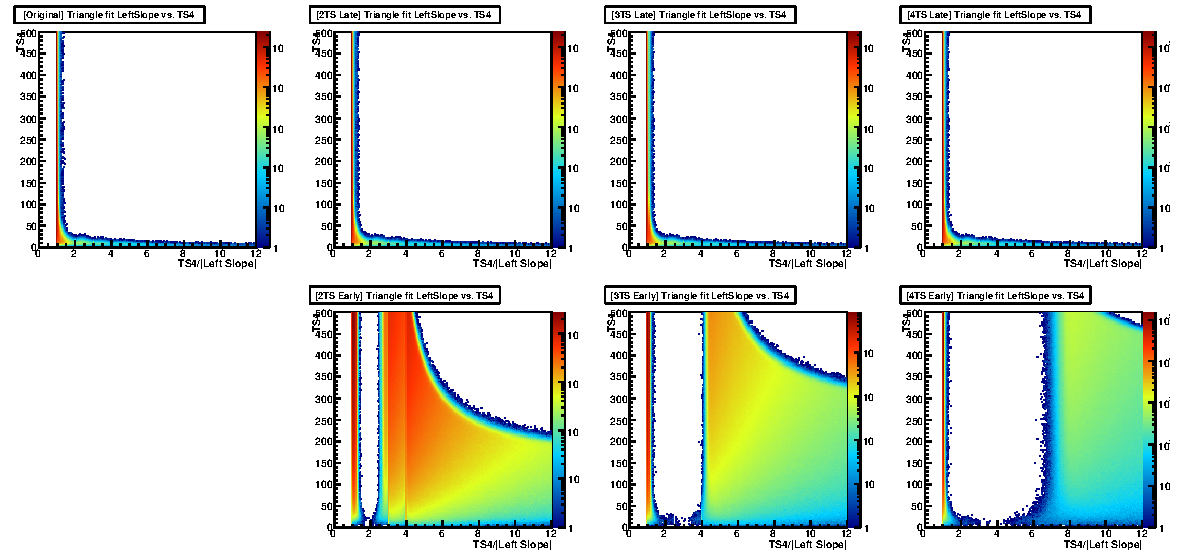
\includegraphics[width=120mm]{DailyLog/6411/6411_ToysAllChargeLeftSlope.pdf}
   \caption{Left slope in the presence of out-of-time pileup (Toy)}
   \label{Figure_6411_ToysAllChargeLeftSlope}
\end{figure}

\begin{figure}
   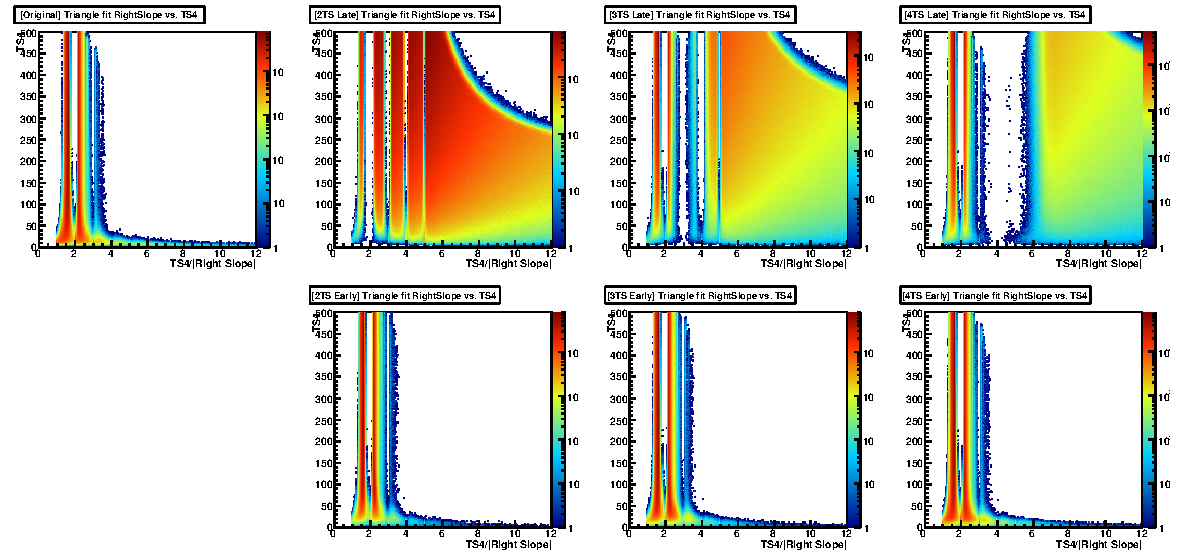
\includegraphics[width=120mm]{DailyLog/6411/6411_ToysAllChargeRightSlope}
   \caption{Right slope in the presence of out-of-time pileup (Toy)}
   \label{Figure_6411_ToysAllChargeRightSlope}
\end{figure}

\begin{figure}
   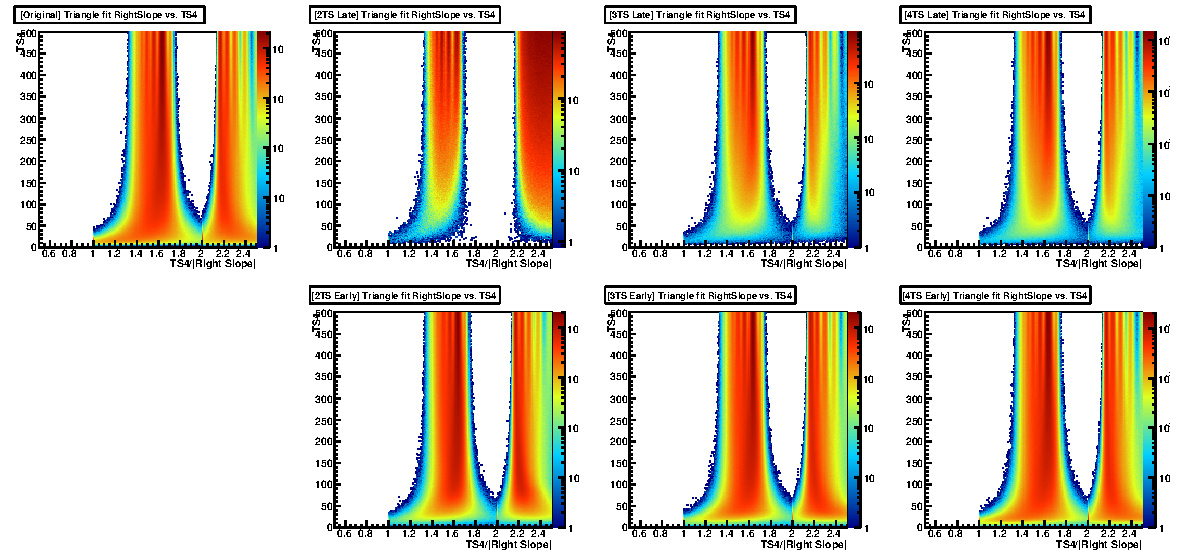
\includegraphics[width=120mm]{DailyLog/6411/6411_ToysAllChargeRightSlopeZoomIn.pdf}
   \caption{Right slope in the presence of out-of-time pileup (Toy)}
   \label{Figure_6411_ToysAllChargeRightSlopeZoomIn}
\end{figure}

\begin{figure}
   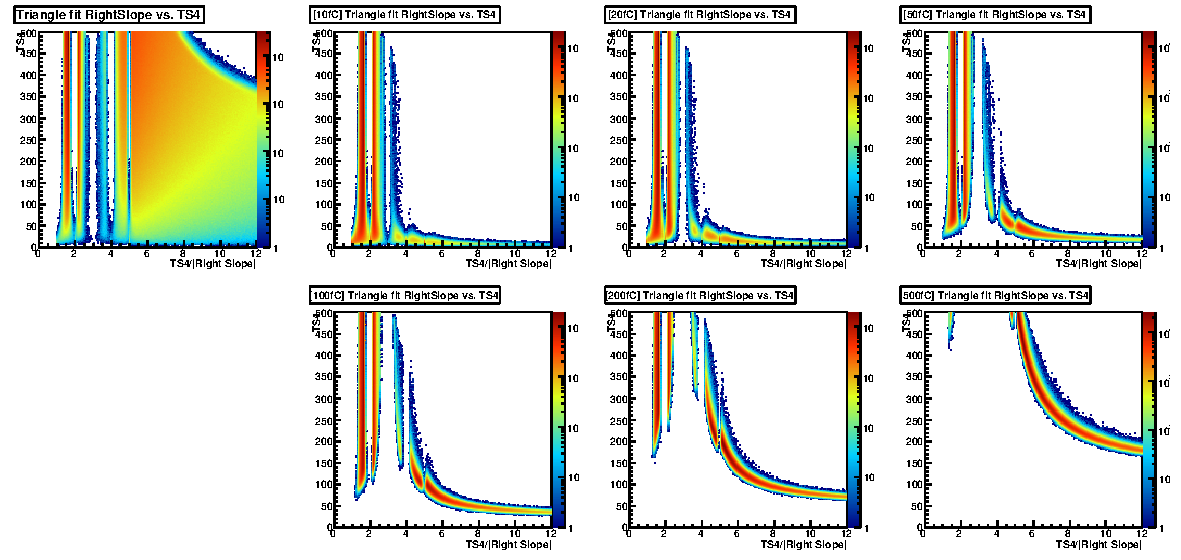
\includegraphics[width=120mm]{DailyLog/6411/6411_Toys75LateScanRightSlope.pdf}
   \caption{Structure in the right slope in the presence of out-of-time pileup (Toy)}
   \label{Figure_6411_Toys75LateScanRightSlope}
\end{figure}

\begin{figure}
   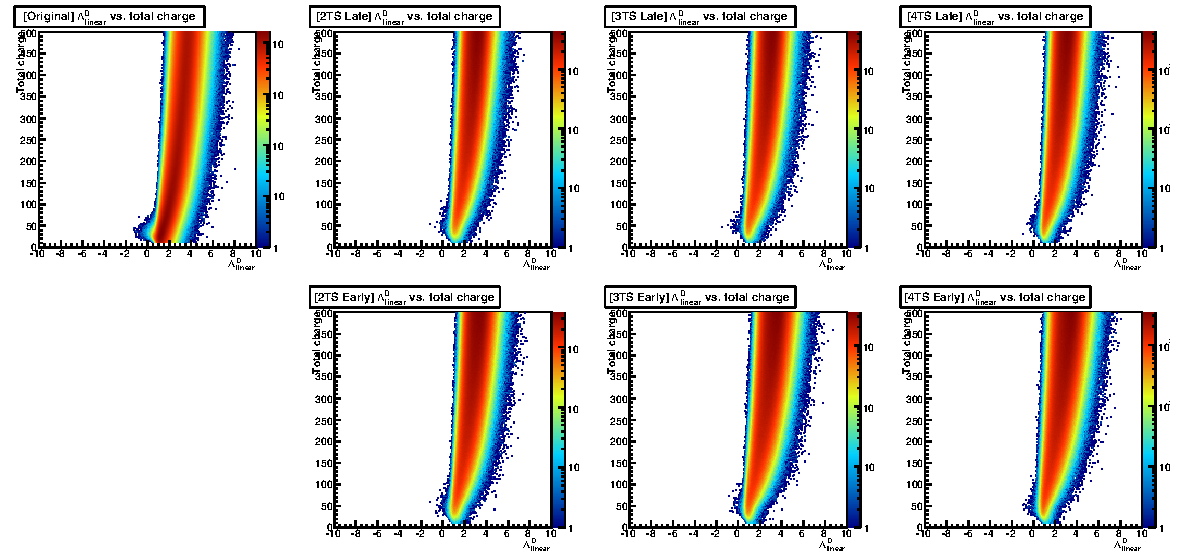
\includegraphics[width=120mm]{DailyLog/6411/6411_ToysAllChargeLambdaDLinear.pdf}
   \caption{Modified linear discriminant (Toy)}
   \label{Figure_6411_ToysAllChargeLambdaDLinear}
\end{figure}

\begin{figure}
   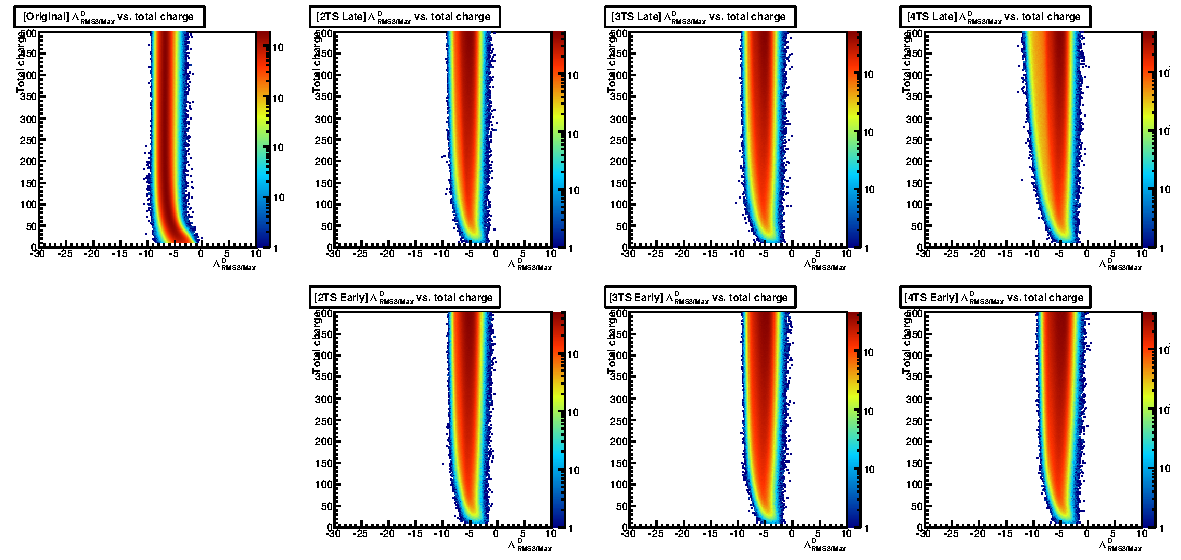
\includegraphics[width=120mm]{DailyLog/6411/6411_ToysAllChargeLambdaDRMS8Max.pdf}
   \caption{Modified spike discriminant (Toy)}
   \label{Figure_6411_ToysAllChargeLambdaDRMS8Max}
\end{figure}

\begin{figure}
   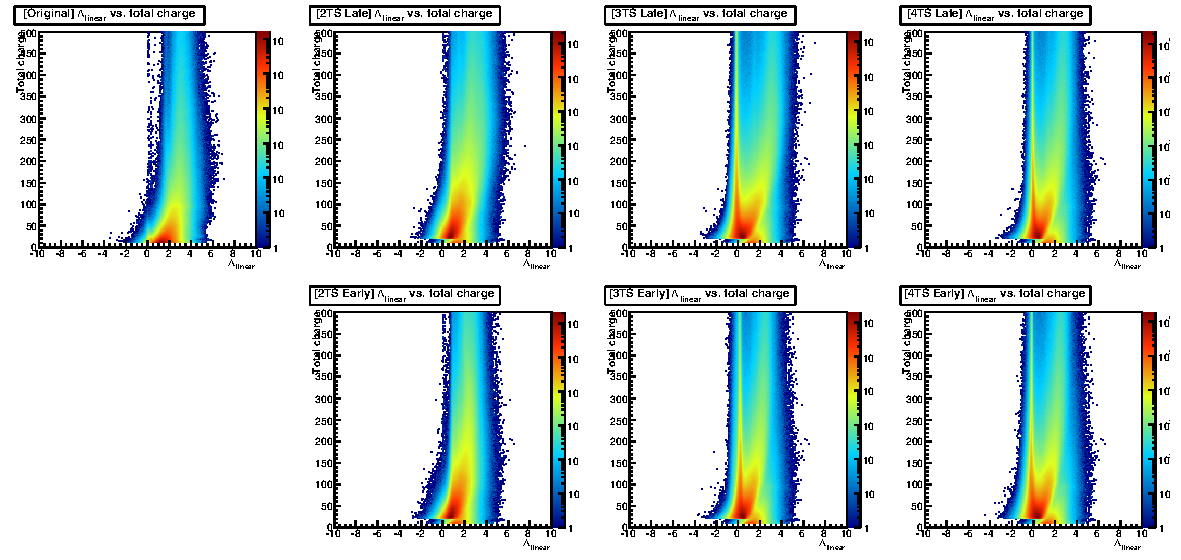
\includegraphics[width=120mm]{DailyLog/6411/6411_MixJetOnJetLambdaLinear.pdf}
   \caption{Linear discriminant (Jet+Jet)}
   \label{Figure_6411_MixJetOnJetLambdaLinear}
\end{figure}
\begin{figure}
   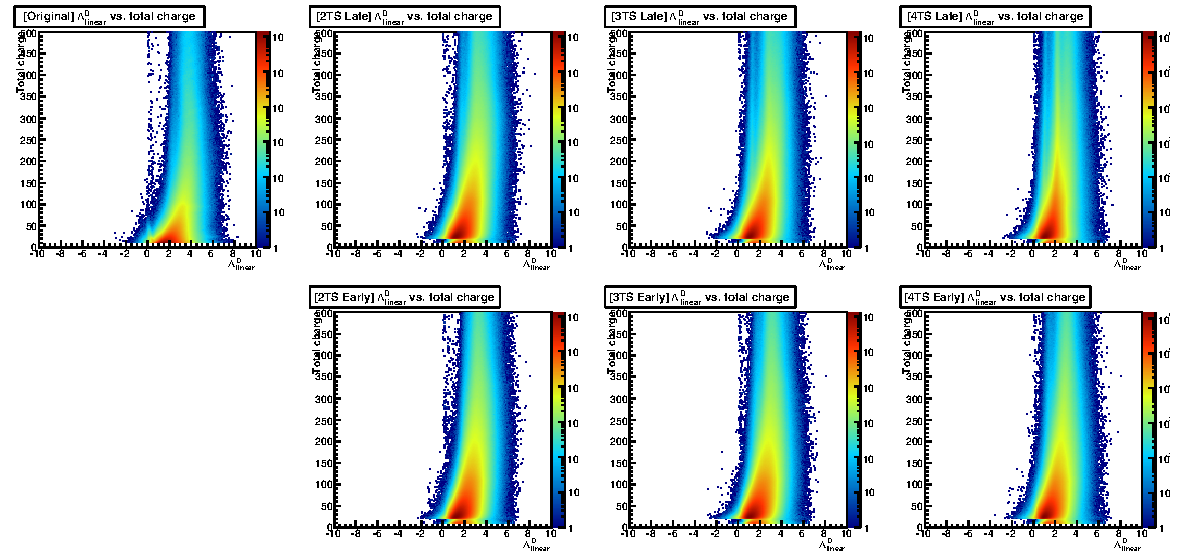
\includegraphics[width=120mm]{DailyLog/6411/6411_MixJetOnJetLambdaDLinear.pdf}
   \caption{Modified linear discriminant (Jet+Jet)}
   \label{Figure_6411_MixJetOnJetLambdaDLinear}
\end{figure}

\begin{figure}
   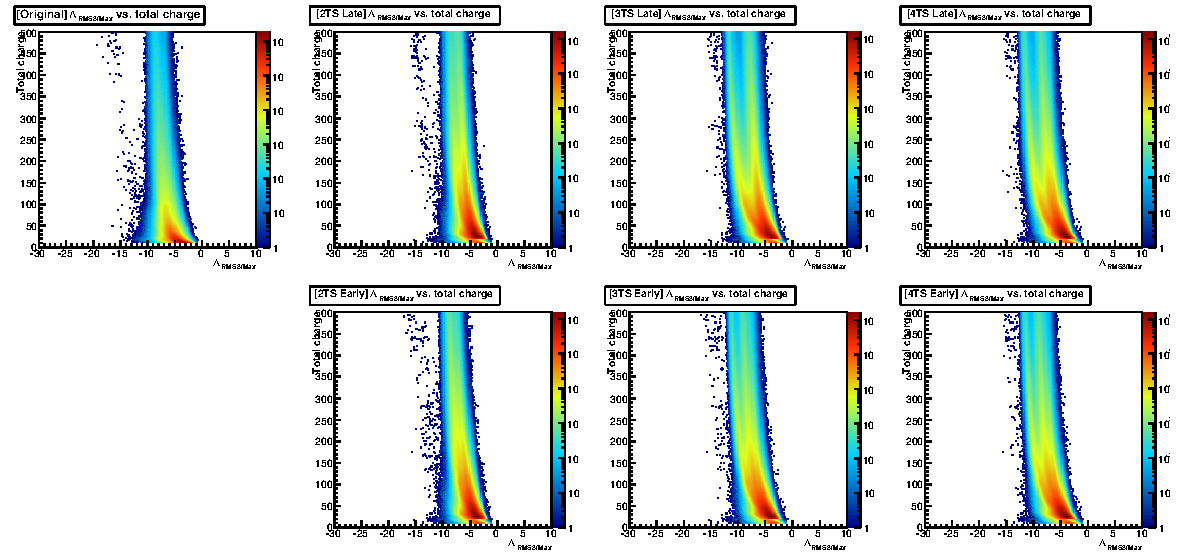
\includegraphics[width=120mm]{DailyLog/6411/6411_MixJetOnJetLambdaRMS8Max.pdf}
   \caption{Spike discriminant (Jet+Jet)}
   \label{Figure_6411_MixJetOnJetLambdaRMS8Max}
\end{figure}
\begin{figure}
   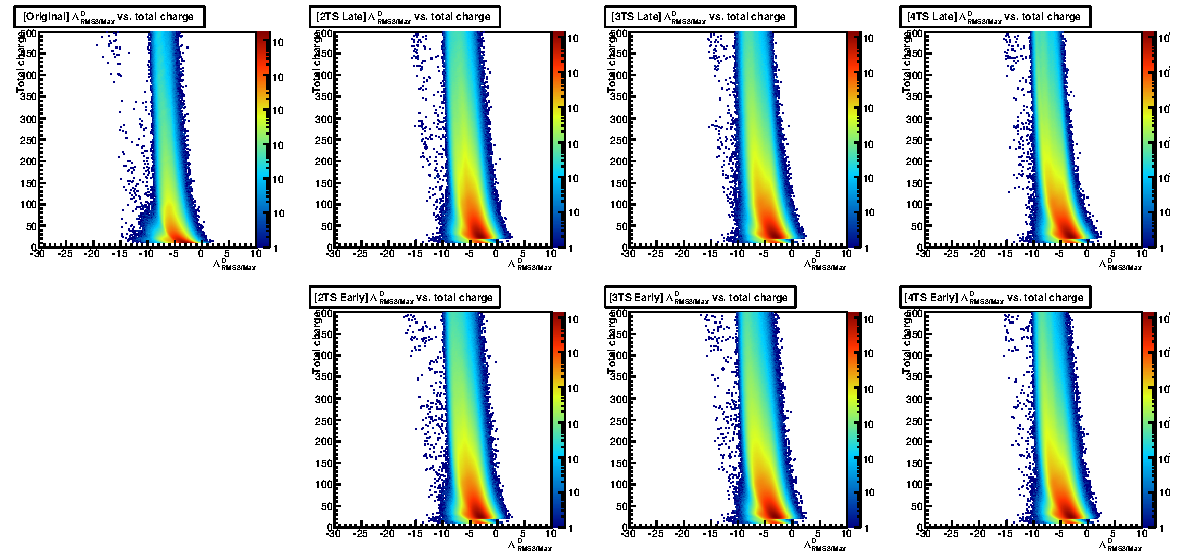
\includegraphics[width=120mm]{DailyLog/6411/6411_MixJetOnJetLambdaDRMS8Max.pdf}
   \caption{Modified spike discriminant (Jet+Jet)}
   \label{Figure_6411_MixJetOnJetLambdaDRMS8Max}
\end{figure}

\begin{figure}
   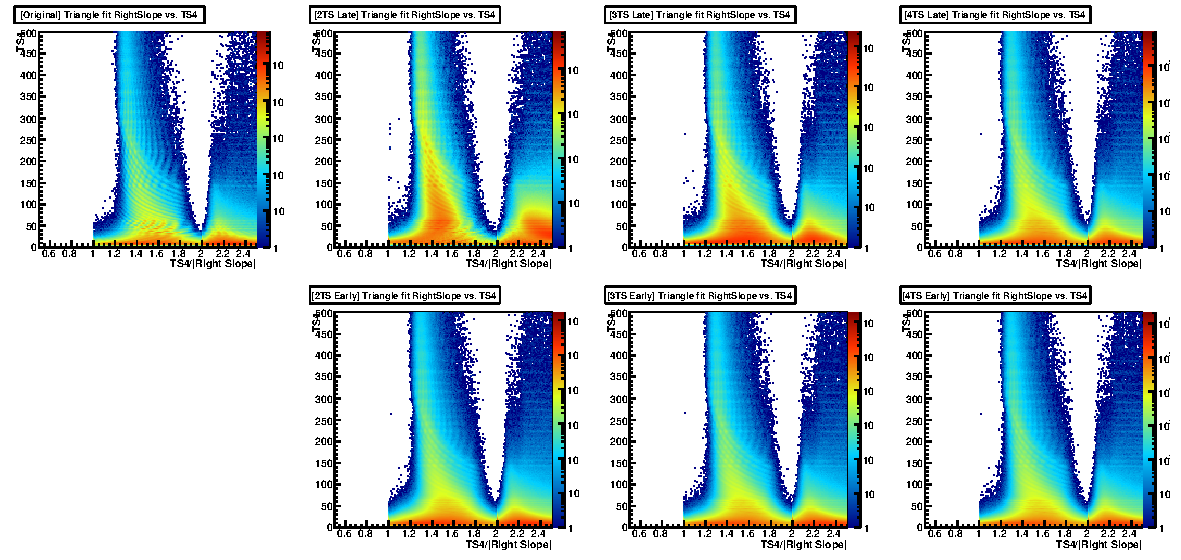
\includegraphics[width=120mm]{DailyLog/6411/6411_MixJetOnJetRightSlopeZoomIn.pdf}
   \caption{(Jet+Jet)  Right slope lower edge looks OK.}
   \label{Figure_6411_MixJetOnJetRightSlopeZoomIn}
\end{figure}

\begin{figure}
   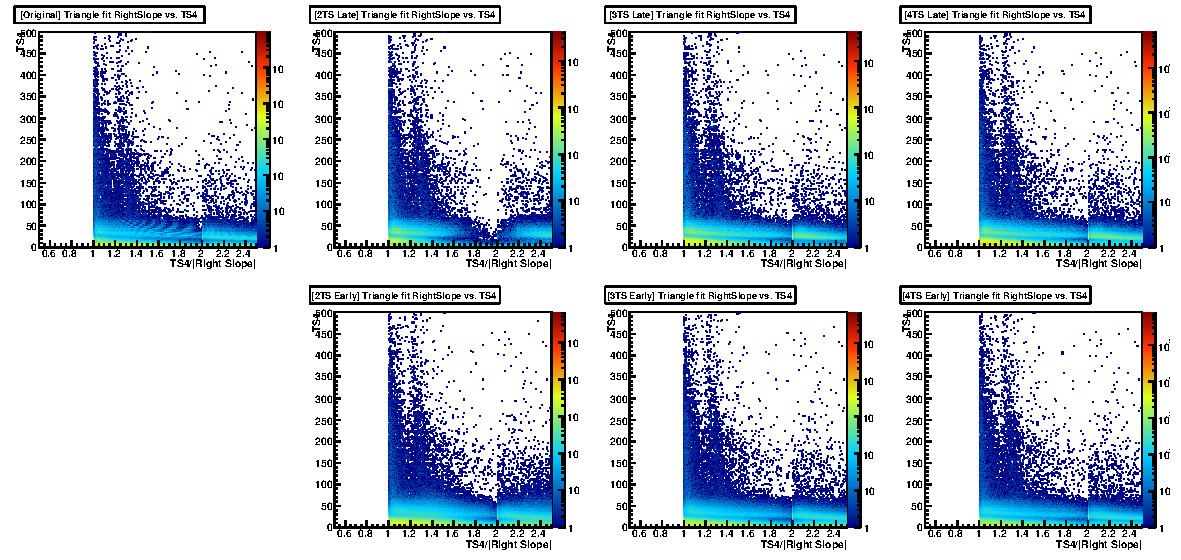
\includegraphics[width=120mm]{DailyLog/6411/6411_MixNoiseOnJetRightSlopeZoomIn.pdf}
   \caption{(Noise+Jet)  Right slope lower edge population still there}
   \label{Figure_6411_MixNoiseOnJetRightSlopeZoomIn}
\end{figure}

\begin{figure}
   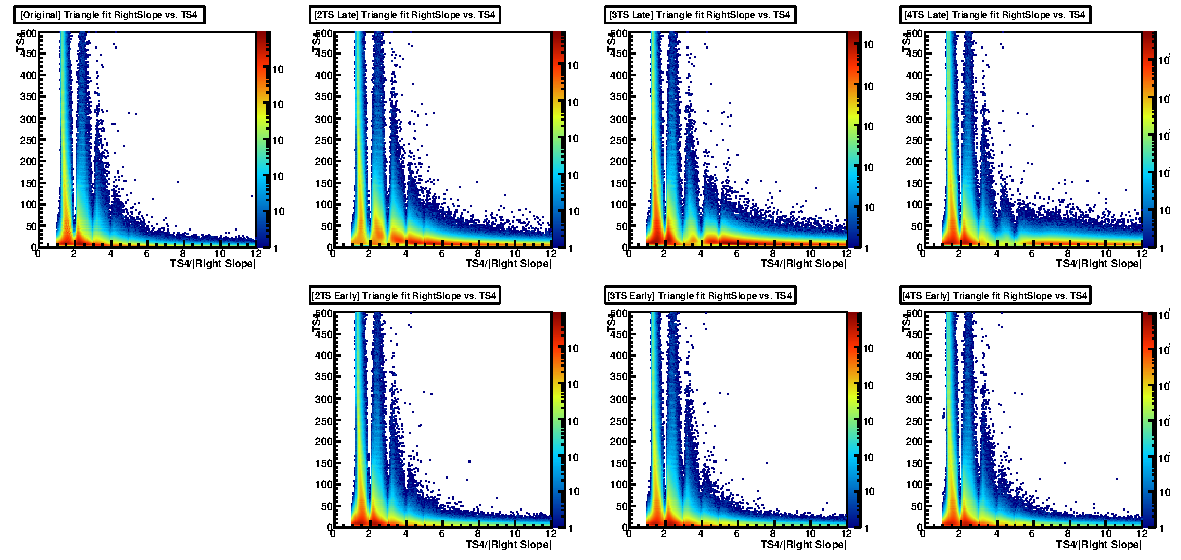
\includegraphics[width=120mm]{DailyLog/6411/6411_MixJetOnMBRightSlope}
   \caption{(Jet+MB) Minimum bias spectrum too soft....}
   \label{Figure_6411_MixJetOnMBRightSlope}
\end{figure}

\begin{figure}
   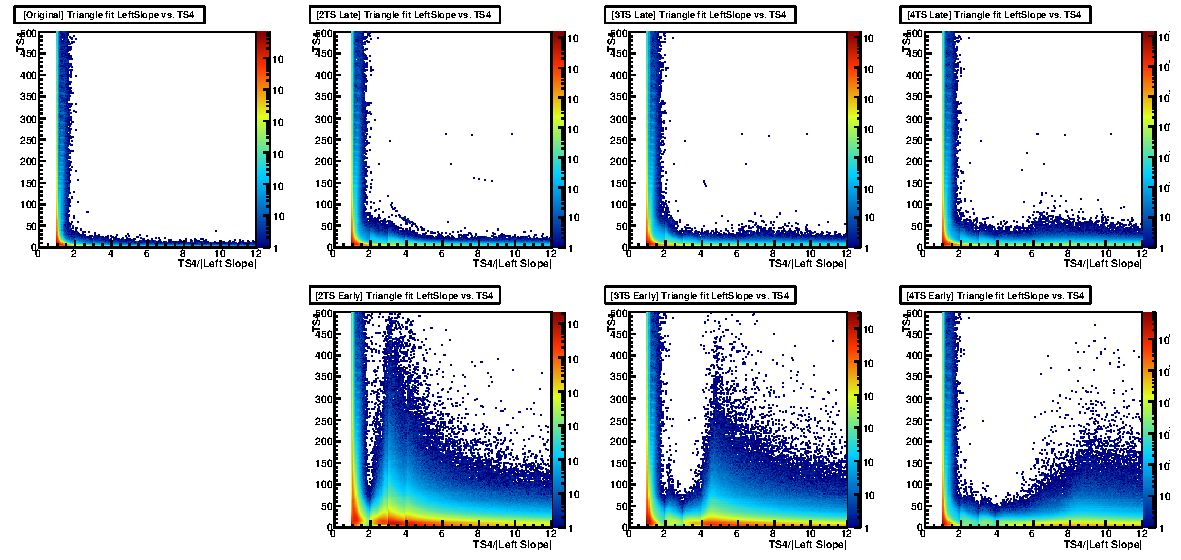
\includegraphics[width=120mm]{DailyLog/6411/6411_MixJetOnJetLeftSlope.pdf}
   \caption{(Jet+Jet) Left slope.}
   \label{Figure_6411_MixJetOnJetLeftSlope}
\end{figure}
\begin{figure}
   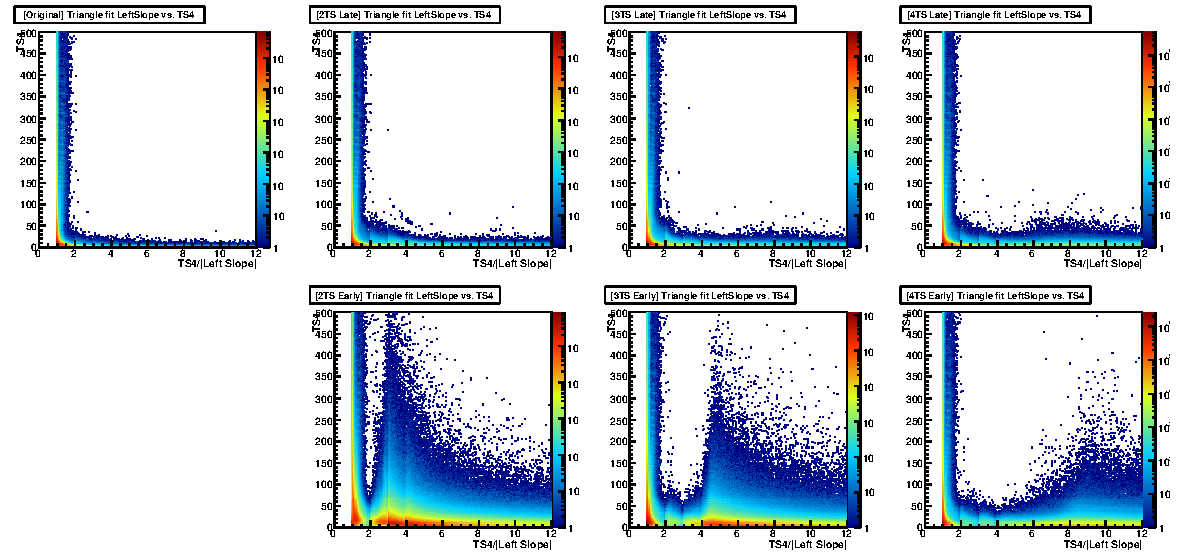
\includegraphics[width=120mm]{DailyLog/6411/6411_MixJetOnMultiJetLeftSlope.pdf}
   \caption{(Jet+MultiJet) Left slope.}
   \label{Figure_6411_MixJetOnMultiJetLeftSlope}
\end{figure}

